\documentclass[usenames,dvipsnames]{beamer}

\mode<presentation> {

% The Beamer class comes with a number of default slide themes
% which change the colors and layouts of slides. Below this is a list
% of all the themes, uncomment each in turn to see what they look like.

%\usetheme{default}
% \usetheme{AnnArbor}
%\usetheme{Antibes}
%\usetheme{Bergen}
% \usetheme{Berkeley}
% \usetheme{Berlin}
%\usetheme{Boadilla}
%\usetheme{CambridgeUS}
% \usetheme{Copenhagen}
\usetheme{Darmstadt}
% \usetheme{Dresden}
% \usetheme{Frankfurt}
% \usetheme{Goettingen}
%\usetheme{Hannover}
%\usetheme{Ilmenau}
%\usetheme{JuanLesPins}
%\usetheme{Luebeck}
% \usetheme{Madrid}
% \usetheme{Malmoe}
%\usetheme{Marburg}
% \usetheme{Montpellier}
% \usetheme{PaloAlto}
% \usetheme{Pittsburgh}
%\usetheme{Rochester}
% \usetheme{Singapore}
%\usetheme{Szeged}
%\usetheme{Warsaw}

% As well as themes, the Beamer class has a number of color themes
% for any slide theme. Uncomment each of these in turn to see how it
% changes the colors of your current slide theme.

% \usecolortheme{albatross}
%\usecolortheme{beaver}
%\usecolortheme{beetle}
%\usecolortheme{crane}
%\usecolortheme{dolphin}
%\usecolortheme{dove}
%\usecolortheme{fly}
\usecolortheme{lily}
%\usecolortheme{orchid}
%\usecolortheme{rose}
%\usecolortheme{seagull}
%\usecolortheme{seahorse}
%\usecolortheme{whale}
%\usecolortheme{wolverine}

%\setbeamertemplate{footline} % To remove the footer line in all slides uncomment this line
%\setbeamertemplate{footline}[page number] % To replace the footer line in all slides with a simple slide count uncomment this line

\setbeamertemplate{navigation symbols}{} % To remove the navigation symbols from the bottom of all slides uncomment this line
}

% % -------------------------------------------
% % Songkai added, feel free to delete --------
% \AtBeginSection[]{
%   \begin{frame}
%   \vfill
%   \centering
%   \begin{beamercolorbox}[sep=8pt,center,shadow=false,rounded=true]{title}
%     \usebeamerfont{title}\insertsectionhead\par%
%   \end{beamercolorbox}
%   \vfill
%   \end{frame}
% }
% % Songkai added, feel free to delete --------
% % -------------------------------------------




\usepackage{graphicx} % Allows including images
\usepackage{booktabs} % Allows the use of \toprule, \midrule and \bottomrule in tables
\usepackage{natbib}
\usepackage{amsmath, amssymb, graphicx, url}
\usepackage[ruled]{algorithm2e}
\usepackage{commath}
\usefonttheme[onlymath]{serif}

\usepackage{amsmath}
\usepackage{amssymb}
\usepackage{centernot}
\usepackage{comment}
%\usepackage[a4paper, margin=0.8in]{geometry}
\usepackage{parskip}
\usepackage{graphicx}

\usepackage{natbib}

\usepackage{tikz}
\usepackage{tikzlings}

\usepackage{tabularx}
\usepackage{array}
\usepackage{multirow}
\usepackage{makecell}
\usepackage{mathtools}
\usepackage{bm,upgreek}
\usepackage{subcaption}
\usepackage{textpos}
% \usepackage{eso-pic}

% \usepackage{multimedia}
\usepackage{media9}

\def\E{\mathbf{E}}
\def\PP{\mathbf{P}}
\def\Reals{\mathbb{R}}
\def\Naturals{\mathbb{N}}
\def\argmin{\operatornamewithlimits{arg\,min}}
\def\deq{:=}
\def\wh#1{\widehat{#1}}
\def\bd#1{\mathbf{#1}}
\def\bx{\bd{x}}
\def\by{\bd{y}}
\def\bZ{\bd{Z}}
\def\bB{\bd{B}}
\def\bV{\bd{V}}
\def\tO{{\tilde{\cO}}}
\def\tOm{\tilde{\Omega}}
\def\barw{\overline{w}}
\def\d{{\mathrm d}}
\def\ave#1{\langle #1 \rangle}
\def\Ave#1{\left\langle #1 \right\rangle}
\def\eps{\varepsilon}
\def\tr{\mathrm{Tr}}


\def\HS{\mathbb{H}}
\def\reals{\mathbb{R}}
\def\ths{\theta^*}
\def\thh{\hat{\theta}}
\def\lbr{\left[}
\def\rbr{\right]}
\def\lc{\left(}
\def\rc{\right)}


    \def\ddefloop#1{\ifx\ddefloop#1\else\ddef{#1}\expandafter\ddefloop\fi}
    % \cA, \cB, ...
    \def\ddef#1{\expandafter\def\csname c#1\endcsname{\ensuremath{\mathcal{#1}}}}
    \ddefloop ABCDEFGHIJKLMNOPQRSTUVWXYZ\ddefloop
    \def\argmin{\operatornamewithlimits{arg\,min}}
    \def\E{\mathbf{E}}
    \def\bx{\bd{x}}
	\def\by{\bd{y}}
    \def\bZ{\bd{Z}}

\newcommand{\propnumber}{} % initialize
\newtheorem*{prop}{Proposition \propnumber}
\newenvironment{propc}[1]
  {\renewcommand{\propnumber}{#1}%
   \begin{shaded}\begin{prop}}
  {\end{prop}\end{shaded}}

\newcommand{\crlrnumber}{} % initialize
%\newtheorem*{corollary}{Corollary \crlrnumber}
\newenvironment{corollaryc}[1]
  {\renewcommand{\crlrnumber}{#1}%
   \begin{shaded}\begin{corollary}}
  {\end{corollary}\end{shaded}}

\theoremstyle{definition}
% \newtheorem{definition}




% \setbeamertemplate{headline}{% 
%     \leavevmode%
%     \hbox{%
%         \begin{beamercolorbox}[wd=.4\paperwidth,ht=2.25ex,dp=1ex,right]{section in head/foot}%
%             \usebeamerfont{section in head/foot}\insertshorttitle\hspace*{2ex}
%         \end{beamercolorbox}%
%         \begin{beamercolorbox}[wd=.6\paperwidth,ht=2.25ex,dp=1ex,left]{subsection in head/foot}%
%             \usebeamerfont{section in head/foot}
\includegraphics[height=2ex,keepaspectratio]{Slides/Block_M-Hex.png}\hspace*{2ex}\insertsectionhead
%         \end{beamercolorbox}%
%     }
% }

% \addtobeamertemplate{headline}{}{%
% \begin{textblock*}{100mm}(.85\textwidth,-1cm)
% \Huge\textcolor{white}{\textbf{\TeX}}
% \end{textblock*}}



%----------------------------------------------------------------------------------------
%	TITLE PAGE
%----------------------------------------------------------------------------------------

%%%% TRY WITH TEXTPOS
% \newcommand{\imgblock}{\begin{textblock*}{5cm}(10.5cm,-1.2cm) % {block width} (coords)
%         
\includegraphics[width=1cm]{Slides/Block_M-Hex.png} % loading the image
%     \end{textblock*}
%     }

% \addtobeamertemplate{background}{\imgblock}{}



% \setbeamertemplate{headline}{\hfill
\includegraphics[width=1.5cm]{Slides/Block_M-Hex.png}\hspace{0.2cm}\vspace{-1cm}}

% \logo{
\includegraphics[height=1cm]{Slides/Block_M-Hex.png}}

\addtobeamertemplate{frametitle}{}{%
    \begin{textblock*}{5cm}(10.5cm, -0.8cm)
        
\includegraphics[width=0.9cm]{Block_M-Hex.png} % your logo file here
    \end{textblock*}
}

\definecolor{mycolor}{cmyk}{100, 60, 0, 60}
\definecolor{my_maize}{rgb}{0.9608,0.7137,0.2588}
\definecolor{my_yellow}{rgb}{0.9294,0.8196,0.2706}

% \setbeamercolor{section in head/foot}{fg=cyan}
\setbeamercolor{section in head/foot}{fg=my_maize}

\setbeamercolor{frametitle}{bg=mycolor}
\setbeamercolor{titlelike}{fg=black, bg=yellow}

\usepackage{url}
\usepackage{hyperref}

\usepackage{xcolor}

\hypersetup{pdfauthor={Name},
            colorlinks=true,
            linkcolor={my_yellow},
            % citecolor={blue},
            % linkcolor=[RGB]{0.949, 0.784, 0.035}
            }

% fix inconsistent colors in cite parenthesis (where the closing parenthesis were black instead of the rest of the citecolor!)
% https://github.com/josephwright/beamer/issues/671
\let\oldcite=\cite
\let\oldcitet=\citet
\let\oldcitep=\citep 
\renewcommand{\citet}[2][]{\textcolor{green}{\oldcitet[#1]{#2}}}
\renewcommand{\citep}[2][]{\textcolor{green}{\oldcitep[#1]{#2}}}
\renewcommand{\cite}[2][]{\textcolor{green}{\oldcite[#1]{#2}}}
            

\title[Seminar]{News Round-up}
% \title[Seminar]{An Adaptive Bayesian Method for Covariance Estimation in Multifidelity Estimators}

% and Estimation of Predictive Uncertainties
% The short title appears at the bottom of every slide, the full title is only on the title page

% \author[AJ]{Aniket Jivani}
% \institute[U-M]{Department of Mechanical Engineering, \\ University of Michigan}

\date{\today}

\AtBeginSection[]
{
 \begin{frame}<beamer>
 \frametitle{Plan}
 \tableofcontents[currentsection]
 \end{frame}
}


\begin{document}

\begin{frame}
\titlepage % Print the title page as the first slide
\end{frame}



% \begin{frame}
%  \frametitle{Overview} % Table of contents slide, comment this block out to remove it
%  \tableofcontents % Throughout your presentation, if you choose to use \section{} and \subsection{} commands, these will automatically be printed on this slide as an overview of your presentation
% \end{frame}


\begin{frame}{04/02/2024}

\begin{enumerate}
    \item Thomas presented on Adaptive Covariance Estimation at \href{https://sites.lsa.umich.edu/mssiss/}{MSSISS 2024}
    
    \item Speaking of MSSISS\dots very few application oriented talks, mostly focused on simple use cases and theoretical developments. However, some interesting topics to chew on for future readings, e.g. Shushu Zhang's talk on expected shortfall regression! - \url{https://arxiv.org/pdf/2307.02695.pdf}
    
    (shortfall regression is of great interest in reliability analysis / risk averse design - see this work on \href{https://kiwi.oden.utexas.edu/papers/Certifiable-Risk-based-engineering-design-optimization-Chaudhuri.pdf}{RiBDO})

    \item (last MSSISS mention) Fascinating keynote talk by \href{https://www.microsoft.com/en-us/research/people/davidmr/}{David Rothschild}
\end{enumerate}

\end{frame}

\begin{frame}{04/02/2024}

\begin{enumerate}
    \item Nice ArXiV: \emph{The Elements of Differentiable Programming} \url{https://arxiv.org/abs/2403.14606}
    
    \item Big solar storm on the weekend of 24th March! \href{https://www.nesdis.noaa.gov/news/noaa-satellites-detect-severe-solar-storm}{NOAA}

    \item Coronacast (SWMF vs reality): \url{https://clasp.engin.umich.edu/solar-eclipse-2024/}
\end{enumerate}
\end{frame}

\begin{frame}{04/09/2024}
\begin{enumerate}
    \item SciFM Highlights:
    \begin{itemize}
            \item AuroraGPT - LLM for Science at Argonne \href{https://www.hpcwire.com/2023/11/13/training-of-1-trillion-parameter-scientific-ai-begins/}{HPC Wire}
            
            \item Big hype around neural operators (which I don't share) - \href{https://www.youtube.com/watch?v=y5EJr4ofGOc}{Anima Anandkumar on AI4Science} - The proposal is to use this kind of architecture in foundation models
            
            \item Petros Koumoutsakos (Harvard) - some work on Multi-agent RL can be found \href{https://www.youtube.com/watch?v=QkrICARm34I}{here} and \href{https://www.nature.com/articles/s41467-022-28957-7}{here - SciMARL}
        \end{itemize}
\end{enumerate}

(Money bets on ML reproducing \href{https://www.cambridge.org/core/journals/journal-of-fluid-mechanics/article/vortex-separation-cascades-in-simulations-of-the-planar-flow-past-an-impulsively-started-cylinder-up-to-boldsymbolre100-boldsymbol000/F419F46158B994407F88BFA2A8410080}{these flows} in the next 50 years)

\begin{figure}
    \centering
    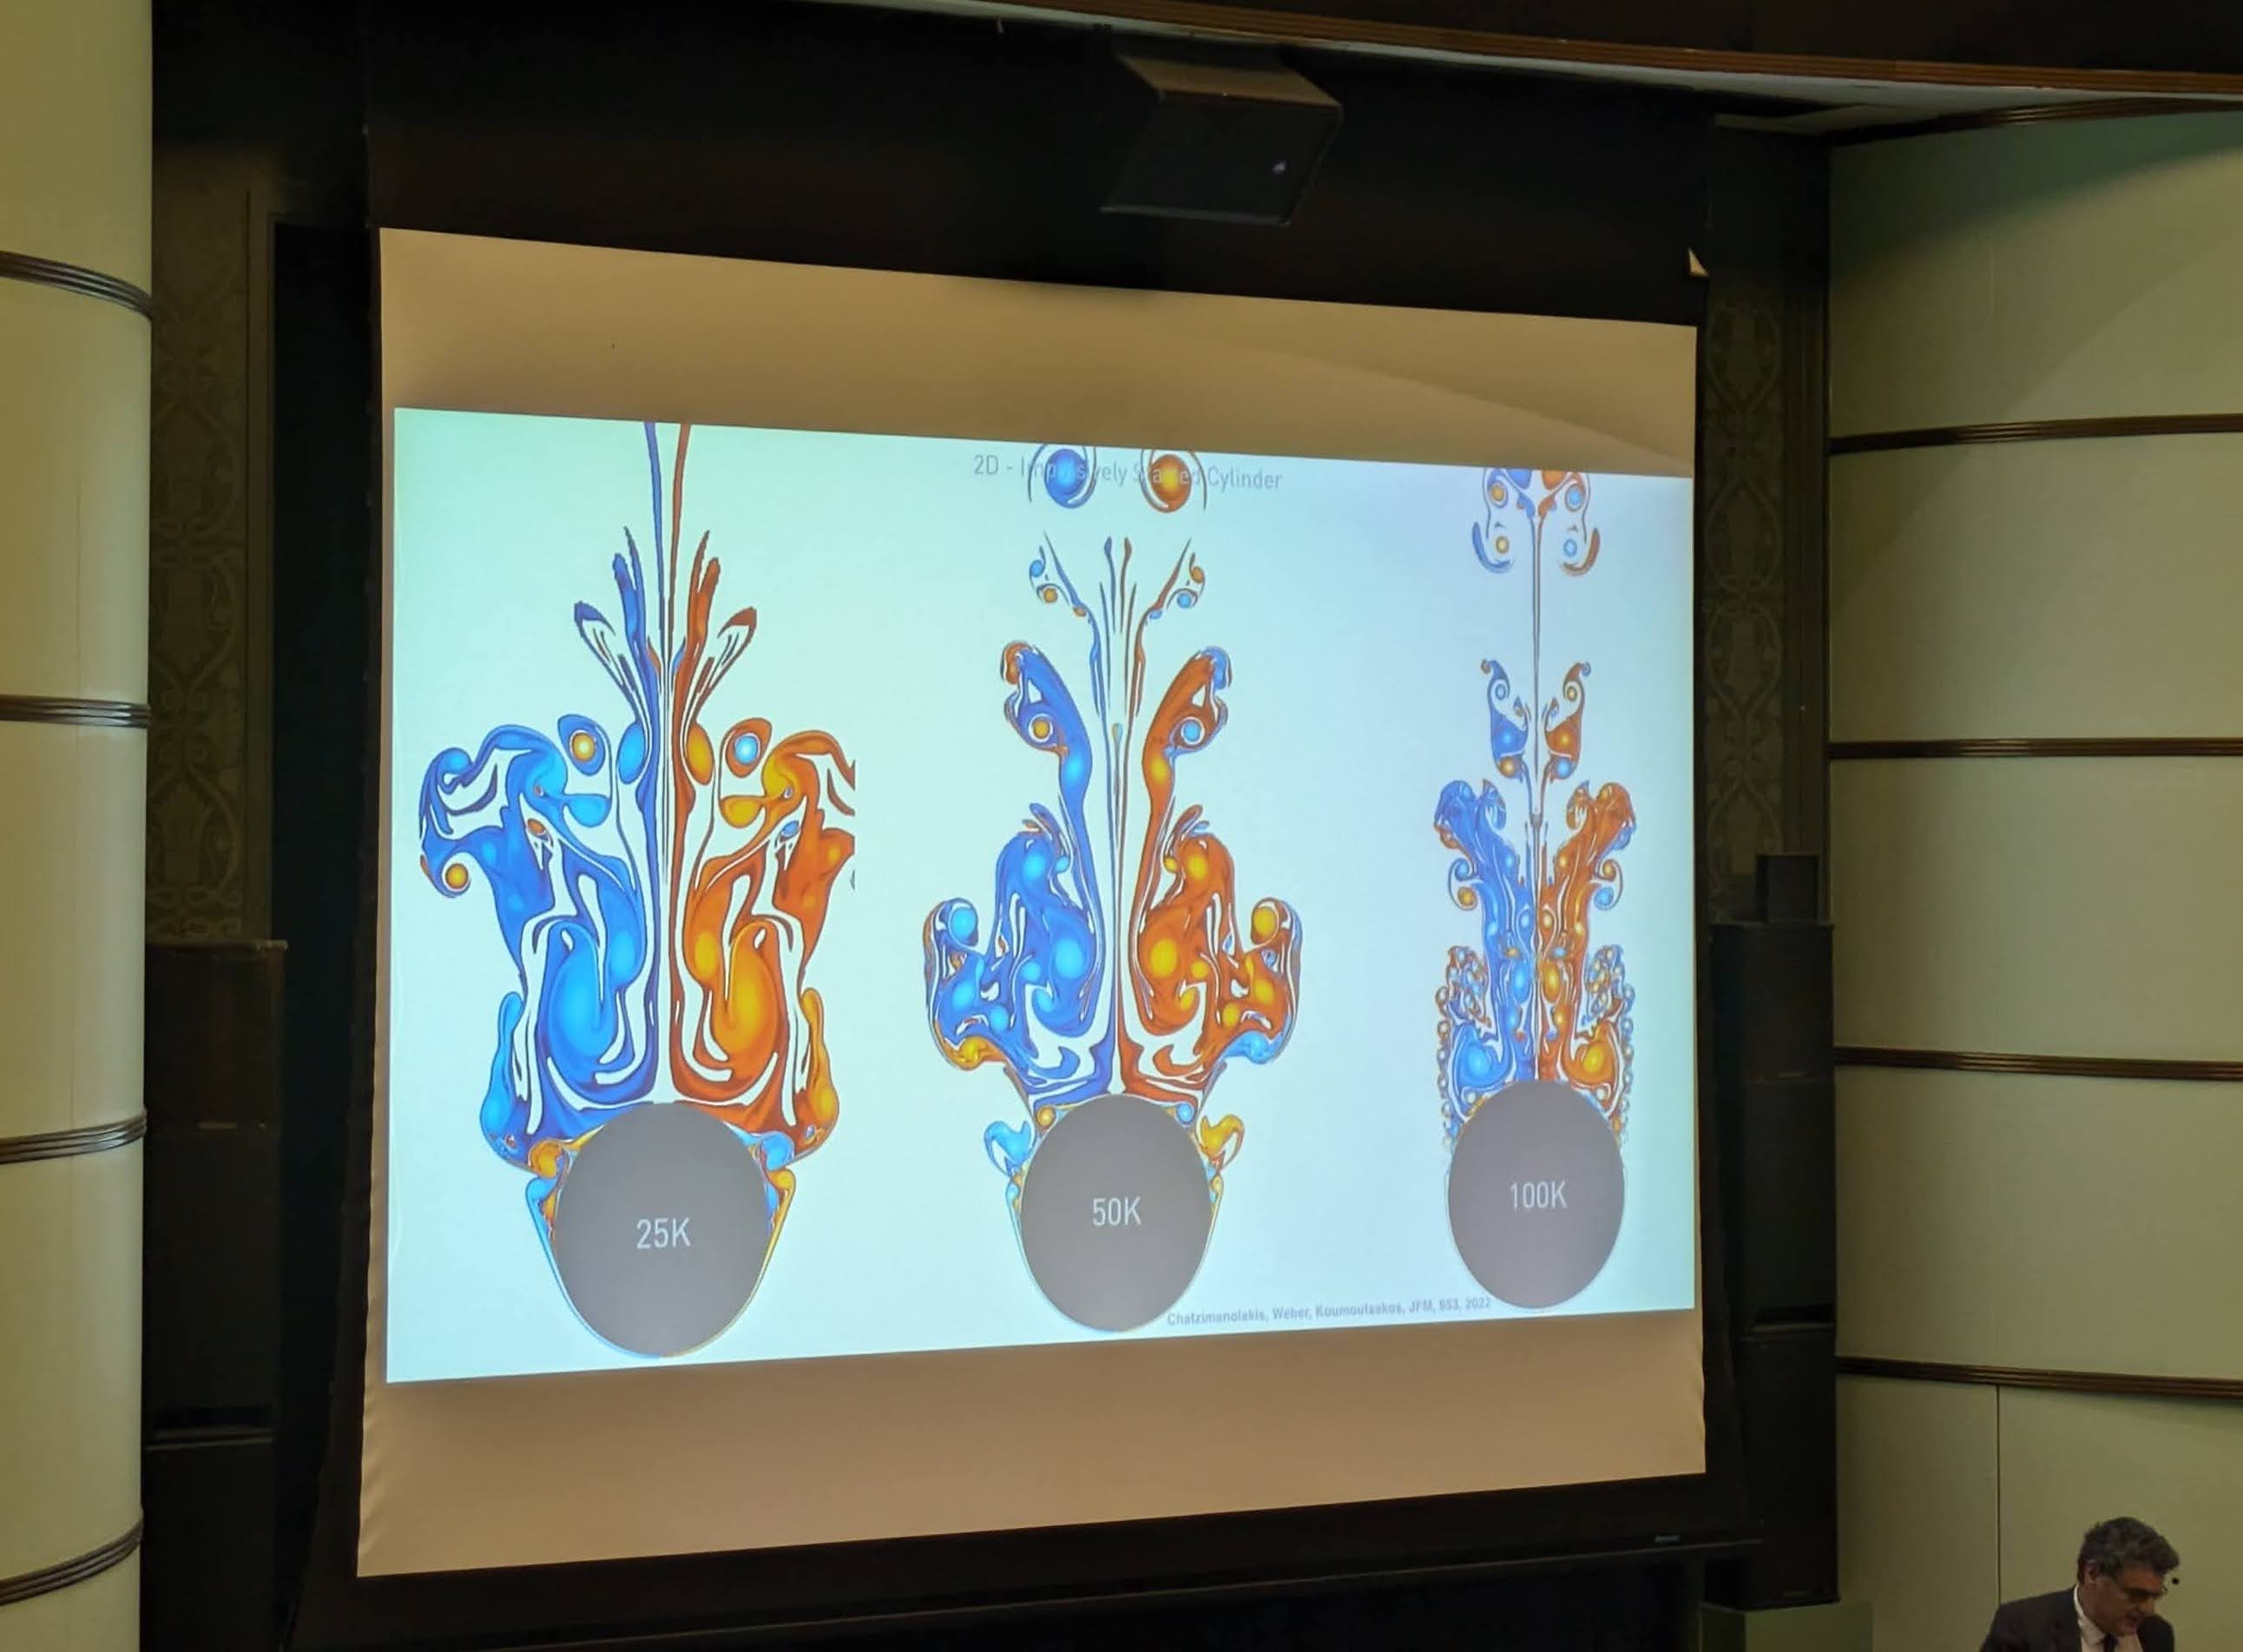
\includegraphics[width=0.45\textwidth]{reproduce_ML.jpg}
    \label{f: reproduce}
\end{figure}
\end{frame}


% \section{Follow up}

% \begin{frame}[allowframebreaks]
%     \frametitle{References}
%     \bibliographystyle{chicago}

%     %\bibliographystyle{IEEEtran}
%     \bibliography{myRef}
% \end{frame}

% \section{Backup}

\begin{frame}{09/17/2024}

\begin{enumerate}
    \item Attended the Model Reduction and Surrogate Modeling Conference (MORe 2024) last week.
    
    \item Very interesting talks - Nested Operator Inference (Nicole Aretz, top secret work that cannot be photographed but paper coming soon), \href{https://kevintcarlberg.net/}{Kevin Carlberg}(Meta), Mariella Kast (Time Evolving NN Parameters Plus Positional Embeddings - \url{https://doi.org/10.1016/j.jcp.2024.112986})
    
    \item One MCMC talk - DINO Acceleration of Geometric MCMC (Lianghao Cao) \url{https://arxiv.org/abs/2403.08220}

    \item Full book of abstracts here:- \url{https://shorturl.at/Jb8Ly}
    
\end{enumerate}
\end{frame}

\begin{frame}
    \begin{figure}[H]
        \centering
        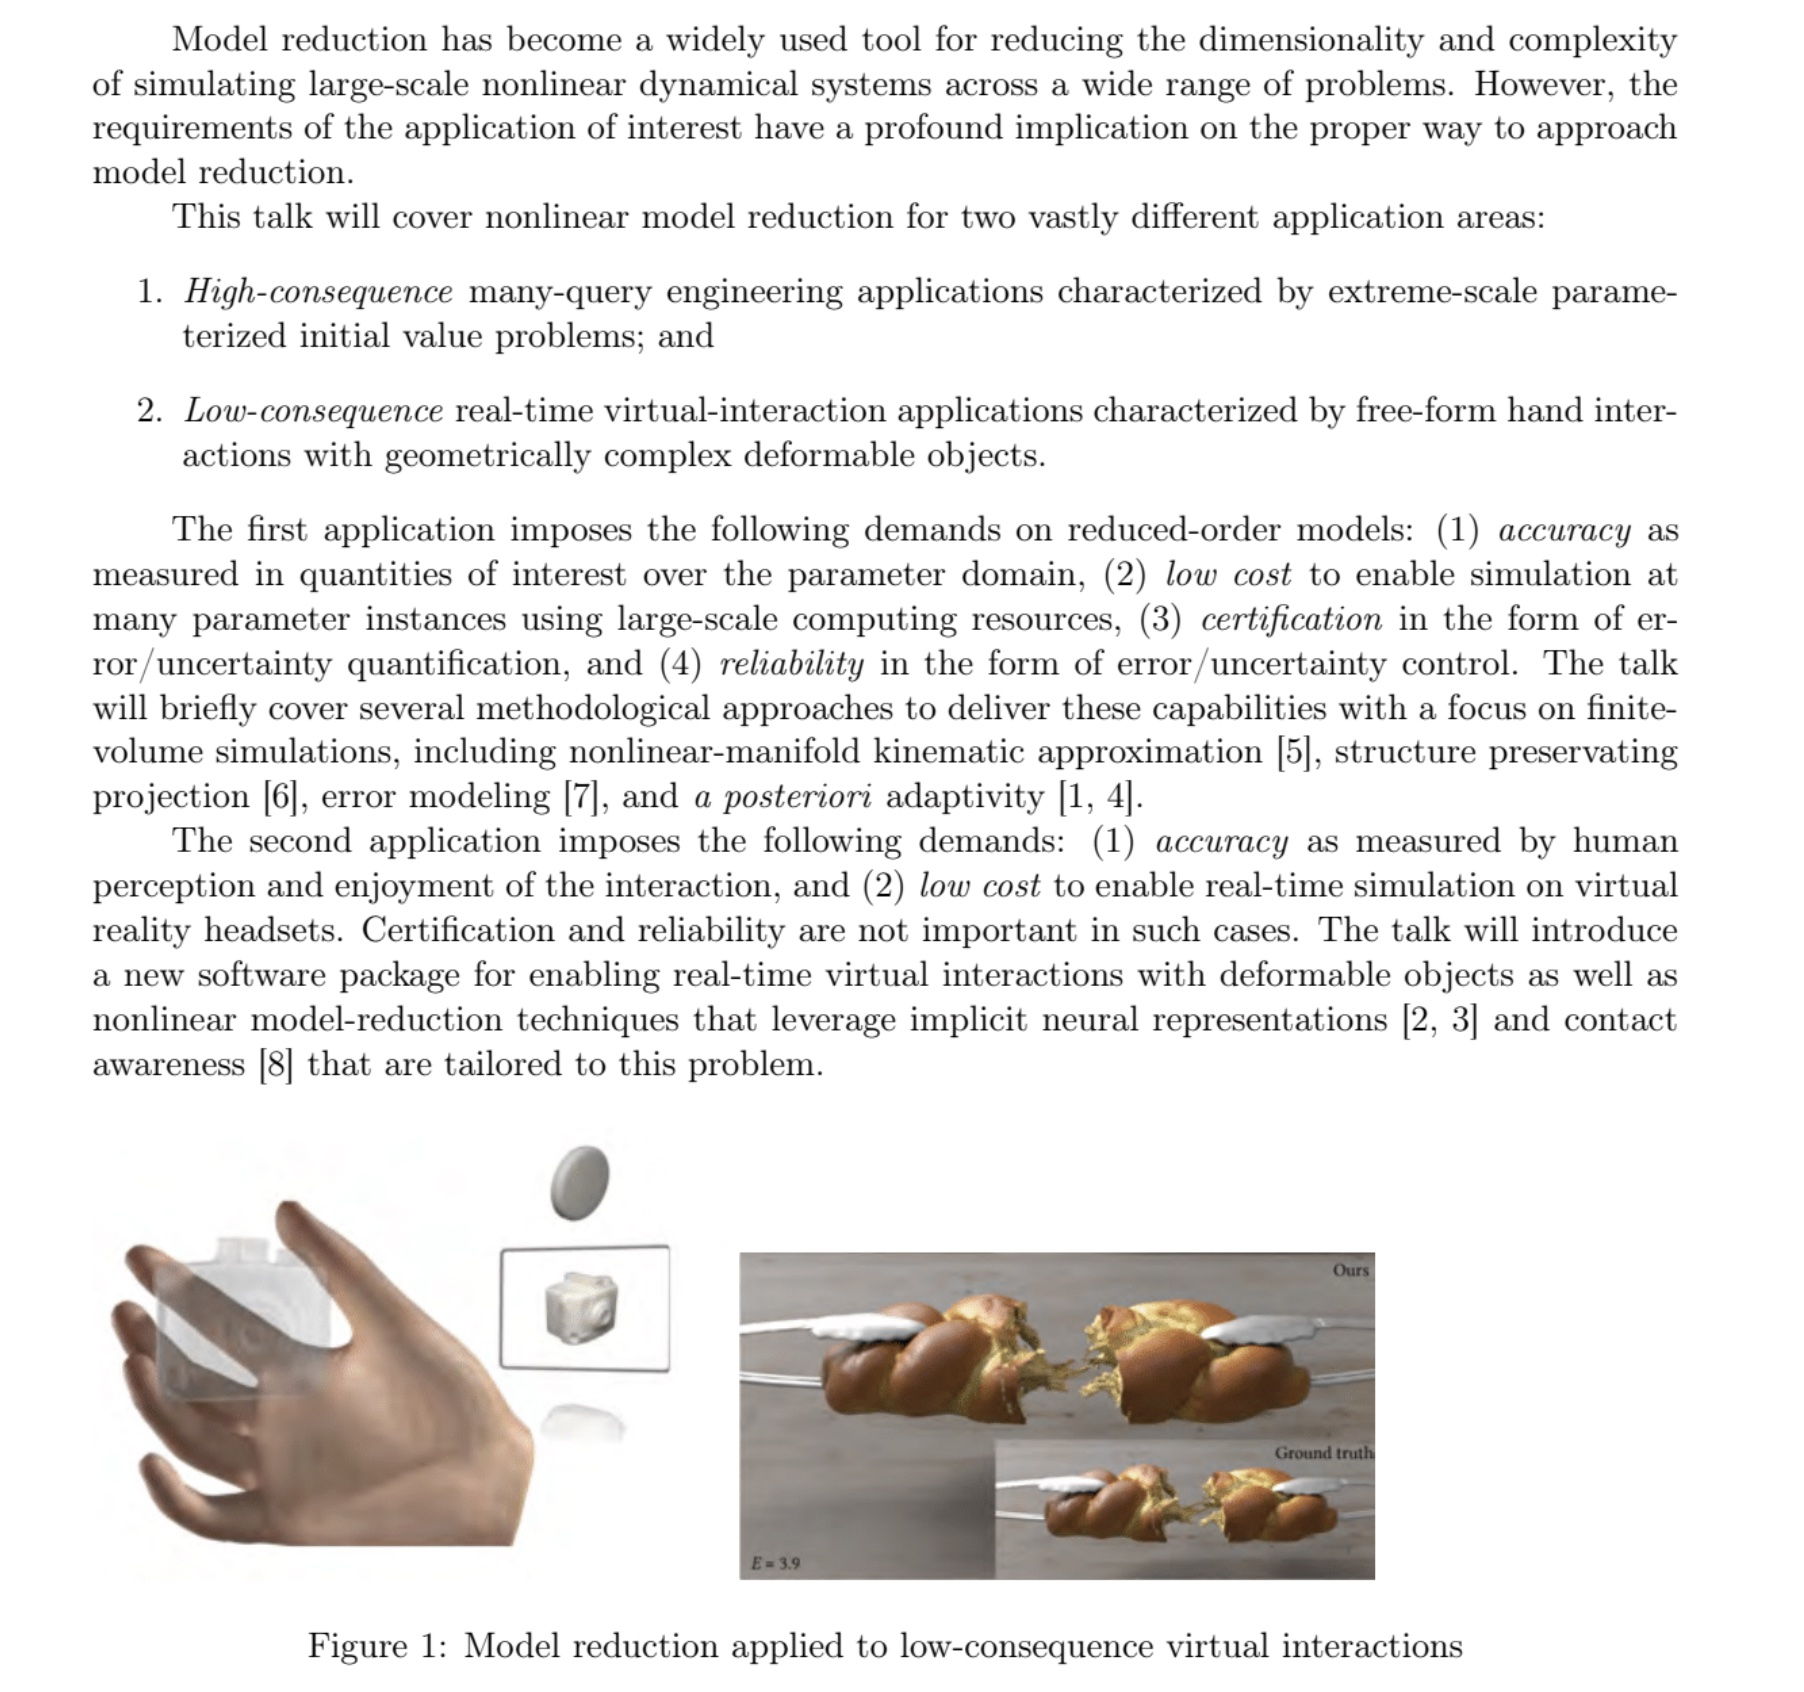
\includegraphics[width=0.9\textwidth]{carlberg_talk_outline.jpg}
    \end{figure}
\end{frame}

\begin{frame}{Upcoming Events}
    \begin{enumerate}
        \item SciML Seminar Series - Starting Sep 20th, every 2 weeks, Friday, 12-1 pm. Limited seating in 2636 GGB + Zoom. (First speaker is Yossi :)

        \item Remaining weeks (Proposal) - regular reading group meetings. Use first meeting (Sep 27, 12-1 pm) to brainstorm (Bring suggestions for papers, vote and select a few)
    \end{enumerate}
\end{frame}

\begin{frame}{}
\begin{center}
    \Large{Thank you!}
\end{center}
        
\end{frame}

\end{document}
